% Thanks to http://tex.stackexchange.com/a/30782/5645 for this
% example!
\documentclass{article}
\usepackage{amsmath}
\usepackage{mathptmx}
\usepackage{tikz}
\usepackage{pgfplots}
\usepgfplotslibrary{polar}
\usepackage{tkz-fct}
\usetikzlibrary{angles, quotes}
\usetikzlibrary{arrows.meta, arrows}
\usetikzlibrary{external}
\tikzexternalize[prefix={external/}]

\tikzset{
    export as png/.style={
        external/system call/.add={}{
            && convert -density #1 -transparent white "\image.pdf" "\image.png"
        },
    },
    export as png/.default={200},
}

\DeclareSymbolFont{symbolsb}{OMS}{cmsy}{m}{n}
\SetSymbolFont{symbolsb}{bold}{OMS}{cmsy}{b}{n}
\DeclareSymbolFontAlphabet{\mathcal}{symbolsb}
\definecolor{myblue}{rgb}{0.067,0.529,0.871}
\definecolor{mypurple}{rgb}{0.859,0.071,0.525}
\definecolor{myred}{rgb}{1.0, 0.13, 0.32}
\definecolor{mygreen}{rgb}{0.01, 0.75, 0.24}
\definecolor{myblack}{gray}{0.5}
\definecolor{mygray}{gray}{0.7}

\def\req{\protect\rotatebox{90}{$\scriptstyle=$}}

\begin{document}

\tikzset{export as png}

\tikzsetnextfilename{disco-solido-revolucion}
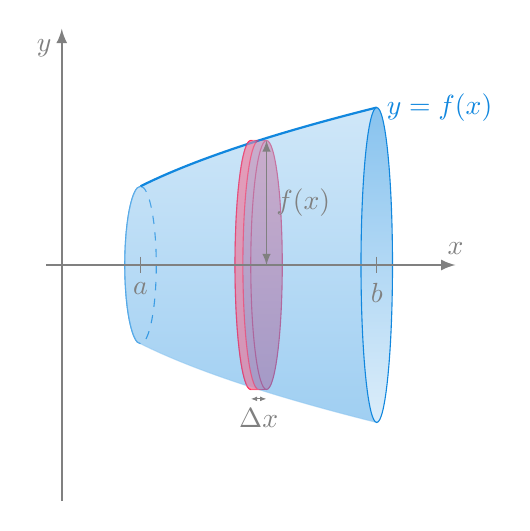
\begin{tikzpicture}[scale=1, >=latex]
    \draw[myred, fill=myred!50] (2.4,0) circle [y radius =1.581138 , x radius =0.2];
    \fill[myred!50] (2.4, -1.581138) rectangle (2.6, 1.581138);
    \draw[myred, fill=myred!50] (2.6, 0) circle [y radius =1.581138 , x radius =0.2];
    \draw[myred] (2.5, 1.581138) -- (2.6, 1.581138);
    \draw[myred] (2.5, -1.581138) -- (2.6, -1.581138);
    \draw[myblue, dashed] (1,1) arc [start angle=90, end angle=-90, x radius=0.2cm, y radius =1cm];
    \draw[myblue] (1,1) arc [start angle=90, end angle=270, x radius=0.2cm, y radius =1cm];
    \shadedraw[myblue!50, shading=axis, top color=myblue!40, bottom color=myblue!80, opacity=0.5] (1,1) -- plot[domain=1:4](\x,{sqrt(\x)}) -- (4,-2) -- plot[domain=4:1](\x,{-sqrt(\x)}) arc [start angle=270, end angle=90, x radius=0.2cm, y radius =1cm];
    \draw[domain=1:4, samples=100, myblue, -, thick] plot (\x, {sqrt(\x)}) node[right] {$y=f(x)$};
    \shadedraw[myblue, shading=axis, top color=myblue!50, bottom color=myblue!15] (4,0) circle [y radius =2 , x radius =0.2];
    \draw[myred, fill = myred!50, opacity=0.5] (2.5,1.581138) -- (2.4, 1.581138) arc [start angle=90, end angle=270, x radius=0.2cm, y radius =1.581138cm] -- (2.5, -1.581138) arc [start angle=270, end angle=90, x radius=0.2cm, y radius =1.581138cm];
    \draw[myblack, {Latex[length=0.8mm]}-{Latex[length=0.8mm]}] (2.4, -1.7) -- (2.6,-1.7) node[below, midway, myblack] {$\Delta x$};
    \draw[myblack, <->] (2.6, 0) -- (2.6, 1.581138) node[right, midway, myblack]  {$f(x)$};
    \draw[->, thick, myblack] (-0.2,0) -- (5,0) node[above] {$x$};
    \draw[->, thick, myblack] (0,-3) -- (0,3) node[below left]{$y$};
    \draw[-, myblack] (1, 3pt) -- (1, -3pt) node[below, myblack] {$a$};
    \draw[-, myblack] (4, 3pt) -- (4, -3pt) node[below, myblack] {$b$};
\end{tikzpicture}
\end{document}


